\documentclass[a4paper,14pt]{extarticle}
\usepackage{array,amsmath,fancybox,amsfonts,graphicx,amsthm,amssymb,wasysym,latexsym,slashed,anysize,subfigure,calc}
\usepackage[spanish]{babel}

%modificaciones para que ch funcione con babel
\usepackage{tikz}
\usetikzlibrary{arrows}
\usepackage{chemmacros}
\chemsetup{modules=all}
\chemsetup{formula=chemformula}

\let\chold\ch
\renewcommand\ch[1]{%
    \catcode`<=12
    \catcode`>=12
    \chold{#1}%
    \catcode`<=\active
    \catcode`>=\active
}
\usepackage[utf8]{inputenc}
\usepackage{fancyhdr,float,hyperref}
\usepackage{lettrine}

\usepackage{enumitem}


%fractiones grandes en inline text: inventa un comando \ddfrac
\newcommand\ddfrac[2]{\frac{\displaystyle #1}{\displaystyle #2}}

%lewis y química
\usepackage{chemformula,elements}
%chemformula, provides \ch{} with the !(<below>)(<formula>) syntax and \chlewis;
%elements, provides \elconf and \writeelconf.
%ex:
%\ch{
%  !(\elconf{Li})( "\chlewis{180.}{Li}" ) +
%  !(\elconf{F})( "\chlewis{0.90:180:270:}{F}" )
%   ->
%  !(\writeelconf{2})( Li+ ) +
%  !(\writeelconf{2,2+6})( "\chlewis{0:90:180:270:}{F}" {}- )
%}


%entorno para química: texto y math mode
%\newcommand*\chem[1]{\textup{#1}}
\newcommand*\chem[1]{\ensuremath{\mathrm{#1}}}

%column
\usepackage{multicol}
%uso: \begin{multicols}{3}

%enumitem: configurar listas
\usepackage{enumitem}

%para los entornos de soluciones
\usepackage{mdframed,xcolor,color}
	%uso: 	entorno (begin,end): {mdframed}[backgroundcolor=brown!10] 

%subrayado y highlight. Tiene que estar detrás de usepackage[color]
\usepackage{soul}
	%\textst{normal} 
	\DeclareRobustCommand{\hlcyan}[1]{{\sethlcolor{cyan}\hl{#1}}} %en cyan!
		%\hl{highlighted text} %uso


%tamaños fuentes extra: 8,9,14,17,20
	\usepackage{extsizes}
	
 	%fuente librebaskerville
 	\usepackage[T1]{fontenc}
	\usepackage{librebaskerville}
	
	%fracciones $$ en texto más elaboradas
	 \usepackage{xfrac}
	 
	%permitir que una ecuación larga esté separada por un salto de página
	\allowdisplaybreaks[4]
		
	%gráficos varios 
	\usepackage{graphics}
	
	%fancy tables
	\usepackage{booktabs}
	\usepackage[small,centerlast,up]{caption}

	
	%mejora en la exposición de guarismos
	\usepackage{numprint}
	
\usepackage{everypage,draftwatermark} %Marca de agua
\SetWatermarkText{\vspace*{2cm}

\hspace*{2cm}\parbox{2\textwidth}{\centering DIST.\\B1-FyQ}}
\SetWatermarkScale{1.5}
\SetWatermarkLightness{0.9}

\DeclareMathOperator{\lin}{lin}
\DeclareMathOperator{\id}{\textbf{id}}
\DeclareMathOperator{\modulo}{mod}

\newcommand{\mc}[3]{\multicolumn{#1}{#2}{#3}}
\newcommand{\halmos}{
\vspace*{-1ex}

\begin{flushright}
\rule{1mm}{2.5mm} \end{flushright}
\vspace*{-1.5ex}

}
\renewcommand{\qed}{\halmos}


%versores: %uso: \uveci\ne\hat{\imath}_{\uvec{i}}+\uvec{j}+\uvec{k}$
\usepackage{bm}
\newcommand{\uveci}{{\bm{\hat{\textnormal{\bfseries\i}}}}}
\newcommand{\uvecj}{{\bm{\hat{\textnormal{\bfseries\j}}}}}
\DeclareRobustCommand{\uvec}[1]{{%
  \ifcsname uvec#1\endcsname
     \csname uvec#1\endcsname
   \else
    \bm{\hat{\mathbf{#1}}}%
   \fi
}}


%algún nuevo operador
\DeclareMathOperator{\cotan}{cotan}


%para textbf en entorno enumerate
\renewcommand{\labelenumi}{%
 \textbf{\theenumi}.
}

%a4
\marginsize{.5cm}{1cm}{1cm}{1cm}%requiere el paquete anysize,izq,dcha,arriba,abajo

%a5
%\marginsize{1cm}{1cm}{1cm}{.5cm}%requiere el paquete anysize,izq,dcha,arriba,abajo

\newtheorem{teo}{{\sc \textbf{Teorema}}}
\newtheorem{defi}{{\sc \textbf{Definición}}}
\newtheorem{coro}{{\sc \textbf{Corolario}}}


%opening
\title{\textbf{	}}
\date{}
\pagestyle{fancy}
\fancyhead[LO,RE]{{\small DOSSIER DE PROBLEMAS\hspace{1ex} \textbf{2Ev}}}
\fancyhead[RO,LE]{{\small B1-DIST\hspace{2ex} FÍSICA y QUÍMICA}}
%\fancyhead[CO,CE]{Ricardo Torres\\http://tinyurl.com/iesCMGfyq}



\begin{document}
\pagenumbering{gobble}

%gas ideal y mezclas
%disoluciones
%estequiometría: ajuste, reactivo limitante, reactivos en disolución e impuros


\begin{enumerate}
  \setlength\itemsep{1.5em}
    
    
    \item (1 punto) Asumiendo que los gases de los que se habla en los siguiente enunciados pueden aproximarse como gases ideales:
    	\begin{itemize}
    		\item[a)] Calcula \textit{razonadamente} la presión parcial de $\chem{NO_2}$, medida en $mmHg$, en $50$ moles de una mezcla gaseosa equimolar de hexafluoruro de azufre y dióxido de nitrógeno en condiciones normales de presión y temperatura. 
    		%380 Torr
    		\begin{mdframed}[backgroundcolor=brown!10]  
    		Si es una muestra \textit{equimolar} las fracciones molares de cada componente son $\chi_\chem{NO_2}=\chi_\chem{SF_6}=0.5$. Como la mezcla se halla en condiciones normales, la presión es de $1\;atm$ y por tanto $$P_\chem{NO_2}=P_\chem{SF_6}=0.5\;atm\simeq 380\;mmHg.$$
    		\end{mdframed}
    		\item[b)] Dos gases puros, \textit{viz.}: metano y hexafluoruro de azufre, se guardan en sendas ampollas. \textit{Razona} cuál de los dos tendrá más densidad en condiciones estándar de presión y temperatura.
    		%Es más denso el hexafluoruro de azufre
    		\begin{mdframed}[backgroundcolor=brown!10]  
    		La ecuación de estado del gas ideal reza $PV=nRT$. Expresando $n$ en función de la masa de la muestra y la masa molar, $M$, obtenemos la ecuación equivalente $PM=\rho RT$, donde $\rho$ es la densidad del gas. 
    		
    		De esta manera, a iguales condiciones de presión y temperatura, la densidad será tanto mayor cuanto mayor sea la masa molecular. El hexafluoruro de azufre será, entonces, más denso.
    		
    		
    		\end{mdframed}
    	\end{itemize}
    \qed
    
    \newpage
    
    \item (2 puntos) Un recipiente de $20\;mL$ contiene nitrógeno molecular a $25^\circ C$ y $0.8\;atm$; otro de $50\;mL$ contiene helio a la misma temperatura y a una presión de $0.4\;atm$. Tras conectar los dos recipientes a través de un pequeño tubo de volumen despreciable, y considerando ambos gases como ideales, estima \textit{razonadamente}:
    	\begin{itemize}
    		\item[a)] El volumen ocupado por cada gas y las presiones parciales.
    		%el volumen es el mismo e igual al total disponible; pN2~0,23 atm; pHe=0,29 atm
    		\begin{mdframed}[backgroundcolor=brown!10]  
    		El volumen es el mismo para cada una de las dos componentes e igual a la suma de los volúmenes de cada recipiente (despreciamos, como nos indican, el volumen del conector). 
    		\vspace{1ex}
    		
    		Aunque no es estrictamente necesario, voy a resolver el problema formalmente, sin usar números: de esta forma podremos ver con claridad qué está sucediendo sin emborronar los pasos.
    		\vspace{1ex}
    		
    		Para calcular las presiones parciales calculamos primero el número de moles de cada componente de la mezcla. A partir de las ecuaciones que describen el estado de cada gas antes de unir los recipientes obtenemos
    		$P_1V_1=n_1RT,\hspace{1.5ex} P_2V_2=n_2RT,$
    		de donde puede despejarse $n_1$ y $n_2$.     		Las fracciones molares serán 
    		\vspace{-3ex}
    		
			\begin{eqnarray*}
				\chi_1&\equiv&\frac{n_1}{n_1+n_2}=\ddfrac{\frac{P_1V_1}{RT}}{\frac{P_1V_1}{RT}+\frac{P_2V_2}{RT}}=\frac{P_1V_1}{P_1V_1+P_2V_2},\\
				\chi_2&\equiv&\frac{n_2}{n_1+n_2}=\ddfrac{\frac{P_2V_2}{RT}}{\frac{P_1V_1}{RT}+\frac{P_2V_2}{RT}}=\frac{P_2V_2}{P_1V_1+P_2V_2},
			\end{eqnarray*}		
			\vspace{-1.5ex}
				    		
    		que suman la unidad, como debe ser.   		Después de mezclar los gases, y aplicando la ecuación de gas ideal al conjunto, podemos escribir la presión total como
    		$$P_TV_T=n_TRT\rightarrow P_T=\left(\frac{P_1V_1}{RT}+\frac{P_2V_2}{RT}\right)\frac{RT}{V_1+V_2}=\frac{P_1V_1+P_2V_2}{V_1+V_2},$$ 
    		de modo que, en virtud de la ley de Dalton,
    		\begin{eqnarray*}
    		P_\chem{N_2}=\chi_1P_T=\frac{P_1V_1}{P_1V_1+P_2V_2}\left(\frac{P_1V_1+P_2V_2}{V_1+V_2}\right)=\frac{V_1}{V_1+V_2}\;P_1\simeq 0.23\;atm,\\
    		P_\chem{He}=\chi_2P_T=\frac{P_2V_2}{P_1V_1+P_2V_2}\left(\frac{P_1V_1+P_2V_2}{V_1+V_2}\right)=\frac{V_2}{V_1+V_2}\;P_2\simeq 0.29\;atm.
    		\end{eqnarray*}
    		%que pueden interpretarse como las presiones de cada componente antes de mezclarse ponderadas a la fracción de volumen, respecto del total, que ocupaban en un principio.
    		\end{mdframed}
    		\newpage
    		
    		\item[b)] La molaridad y el porcentaje en masa de $\chem{He}$ en la disolución.
    		%[He]~1.2E-2 mol/L; %He~15%
    		\begin{mdframed}[backgroundcolor=brown!10]  
    		La molaridad del nitrógeno y el helio en la disolución gasesosa serán, a la vista de los resultados calculados en el apartado a), 
		\[[\chem{He}]\equiv\frac{n_2}{V_1+V_2}=\frac{V_2}{V_1+V_2}\;\frac{P_2}{RT}\simeq 1.2\cdot 10^{-2}\,mol\,L^{-1}. \]
    	Respecto al porcentaje en masa tenemos, aplicando la definición y considerando que la masa de la muestra en función de la masa molar es $m=n\,M$, 
    	\[\%\chem{He}\!=\!\frac{10^2\,m_\chem{He}}{m_\chem{He}+m_\chem{N_2}}\!=\!\frac{10^2\,n_2\,M_\chem{He}}{n_1\,M_\chem{N_2}+n_2\,M_\chem{He}}\!=\!\frac{10^2P_2V_2\,M_\chem{He}}{P_1V_1\,M_\chem{N_2}+P_2V_2\,M_\chem{He}}\simeq 15\%\]
    		\end{mdframed}
    	\end{itemize}
	\qed   
	
	\newpage
	
	
	\item (1 punto) Responde \textit{razonadamente} a las siguientes cuestiones:
		\begin{itemize}
			%\item[a)] ¿Qué volumen debes tomar de una disolución $3\,M$ de ácido nítrico para preparar $500\;cm^3$ de otra que sea $2\,M$ del mismo ácido?
			\item[a)] La etiqueta de una botella de ácido clorhídrico comercial indica una concentración $15.5\,M$ y densidad $1.41\;g\,cm^{-3}$. Calcula su concentración como porcentaje en masa.
			%40,1%
			\begin{mdframed}[backgroundcolor=brown!10]  
			Para hacer el cálculo más sencillo supongamos que tomamos una muestra de $1\;L$ de disolución. Habida cuenta de la densidad, la masa de la muestra será de $1410\;g$ y en ella habrá $15.5\;mol$ de $\chem{HCl}$, que equivalen a $m=n\,M_\chem{HCl}=15.5\cdot 36.5\simeq 568.8\;g.$
			
			Aplicando la definición de porcentaje en masa tendremos
			$$\%\chem{HCl}=\frac{568.8}{1410}\cdot 100\simeq 40.1\%$$
			\end{mdframed}
			\item[b)] Se prepara una disolución con $3\;g$ de $\chem{KCl}$ y $200\;cm^3$ de agua de modo tal que la mezcla resultante tiene una densidad aproximada de $1.02\;g\,cm^{-3}$. Estima su concentración como porcentaje en masa.
			% ~1.5%
			\begin{mdframed}[backgroundcolor=brown!10]  
			Al echar los $3\;g$ de la sal el cambio de volumen será despreciable frente a los $200\;cm^3$, de manera que podemos suponer que la disolución va a tener ese mismo volumen. La masa de esa cantidad de mezcla será $m\simeq\rho\,V=1.02\;g\,cm^{-3}\cdot 200\;cm^3\simeq 204\;g.$
			
			El porcentaje en masa de soluto, entonces, puede escribirse como
			$$\%\chem{KCl}\simeq \frac{3}{204}\cdot 100\simeq 1.5\%$$
			\end{mdframed}
		\end{itemize}
    \qed
    
    \newpage
 
    \item (2 puntos)
    	\begin{itemize}
    		\item[a)] Considera la combustión de gas metano en condiciones normales. \textit{Razona} qué volumen de oxígeno molecular se requiere para quemar completamente $150\;L$ de metano.
    		%300 L
    		\begin{mdframed}[backgroundcolor=brown!10]  
    		Si las condiciones de presión y temperatura no cambian durante la reacción, la estequiometría en moles es totalmente equivalente a la estequiometría en litros (recuerda que la ecuación de estado del gas ideal indica que $\mathbf{n}=\sfrac{P}{RT}\mathbf{V}$ y son, por tanto, proporcionales).
    		
    		La reacción ajustada es 
    		\begin{center}
    		\ch{CH4 + 2 O2 -> CO2 + 2 H2O}
    		\end{center} de manera que por cada mol de metano consumido se requiere el concurso de dos moles de oxígeno molecular. 
			    		
    		Como queremos quemar no uno, sino $150\;L$ es evidente que se necesitaran $300\;L$ de oxígeno molecular.

    		\end{mdframed}
    		\item[b)] Se ponen a reaccionar $100\;g$ de cloruro de bario con $115\;g$ de sulfato de sodio para dar cloruro de sodio y sulfato de bario. Determina \textit{razonadamente} los gramos de sal común que resultan.
    		%56.5 g
    		\begin{mdframed}[backgroundcolor=brown!10]  
    		Una posible representación de la reacción ajustada es 
    		\begin{center}
    			\ch{BaCl2 + Na2SO4 -> 2 NaCl + BaSO4},
    		\end{center}
    		que indica que cloruro de bario y sulfato de sodio reaccionan \textit{uno a uno}. 
    		\vspace{1ex}
    		
    		Veamos cuántos moles tenemos disponibles en las muestras:
    			\begin{itemize}
    				\item $100\;g$ de cloruro de bario son $\sfrac{100}{208}\simeq 0.48\,mol,$
    				\item $115\;g$ de sulfato de sodio son $	\simeq\sfrac{115}{142}\simeq 0.81\,mol.$
				\end{itemize} 
			Como han de reaccionar \textit{uno a uno} está claro que deben reaccionar $ 0.48\,mol$ de cloruro con $ 0.48\,mol$ de sulfato, sobrando $ 0.33\,mol$ de este último. 
			\vspace{1ex}
			
			Según la estequiometría, los moles de sal común obtenidos serán $2\cdot 0.48\simeq 0.96$, equivalentes a una masa de $ 0.96\cdot 58.5\simeq 56\;g$.

    		\end{mdframed}
    	\end{itemize}
    \qed
    
    \newpage
    
    \item (3 puntos) En un laboratorio a $50^\circ\,C$ y $3$ atmósferas de presión se hacen reaccionar $50\;g$ de un mineral de cobre de $90\%$ de pureza con $400\;mL$ de una solución $6\,M$ de ácido nítrico. Sabiendo que el rendimiento para la formación de dióxido de nitrógeno gaseoso es del $95\%$ y que se forma, además, nitrato de cobre{\small (II)} y agua,:
    	\begin{enumerate}[label=\alph*)]
    		\item Escribe y ajusta la reacción.
    		\begin{mdframed}[backgroundcolor=brown!10]  
    		\ch{Cu + 4 HNO3 -> 2 NO2 +  Cu(NO3)2 + 2 H2O}
    		\end{mdframed}
    		\item Identifica \textit{razonadamente }el reactivo limitante y calcula la masa que sobra del reactivo en exceso.
    		%6.6 g
    		\begin{mdframed}[backgroundcolor=brown!10]  
    		Veamos cuántos moles tenemos de cada reactivo: 
    		\begin{itemize}
    			\item En $50\;g$ de mineral con un $90\%$ de pureza hay $45\;g$ de cobre puro, \textit{i.e.} $\sfrac{45}{63.5}\simeq 0.7\;mol$.
    			\item En $400\;mL$ de solución $6\,M$ hay $6\cdot 0.4\simeq 2.4\,mol$ de ácido nítrico puro.
    		\end{itemize}
    		Cobre y ácido nítrico han de reaccionar en proporción $1:4$ de manera que para que los $0.7$ moles de cobre reaccionaran completamente se necesitarían $4\cdot 0.7\simeq 2.8\;mol$ de ácido nítrico. No los hay, de manera que aquel debe ser el reactivo limitante.
    		\vspace{1ex}
    		
    		Reaccionarán, por tanto, $2.4\;mol$ de ácido nítrico con $0.6\;mol$ del metal resultando en un exceso de $0.7-0.6\simeq 0.1\;mol$ de cobre, es decir, $0.1\cdot 63.5\simeq 6.4\;g$.
    		\end{mdframed}
    		\item Suponiendo que se comporta idealmente, calcula \textit{razonadamente} el volumen de dióxido de nitrógeno que se obtiene.
    		%10 L
    		\begin{mdframed}[backgroundcolor=brown!10]  
    		A partir de los $0.6\;mol$ de cobre se formarán, teniendo en cuenta el rendimiento, $2\cdot 0.6\cdot 0.95\simeq 1.1\;mol$ de $\chem{NO_2}$. Si suponemos que se comporta idealmente, en las condiciones prescritas ocupará un volumen de
    		\[V=\frac{nRT}{P}\simeq\frac{1.1\cdot 0.082\cdot 323}{3}\simeq 10\;L.\]
    		\end{mdframed}
    	\end{enumerate}
  	\qed
  	
  	\newpage
  	
  	\item (1 punto) Resuelve \textit{razonadamente} las siguientes cuestiones: 
    	\begin{itemize}
    		\item[a)] El volumen molar, $\bar{v}$, de un gas se define como el volumen que ocupa un mol de gas.   		Calcula en condiciones normales el volumen molar de las siguientes especies gaseosas ideales:  \textit{	i) cloro molecular,\hspace{1ex}ii)  dióxido de azufre; y iii)	    una mezcla equimolar de cloro molecular y dióxido de azufre.}
    		\vspace{2ex}
    		\begin{mdframed}[backgroundcolor=brown!10]  
    		Según la ecuación de estado del gas ideal, en condiciones normales un mol de gas ocupará un volumen de 
    		\[V=\frac{RT}{P}\bigg|_{P=1\,atm,\;T=273\;K}\simeq 22.4\;L,\]
    		\textit{independientemente de la naturaleza del gas}.
    		\end{mdframed}
    		\item[b)] Para caracterizar cómo de bien se ajusta un gas \textit{real} al comportamiento ideal puede utilizarse el llamado \textit{factor de compresibilidad}, $Z$, que se define a través de la expresión $Z\equiv\dfrac{P\,\bar{v}}{RT}.$
    		%		con $\bar{v}$ el volumen molar, definido en el apartado anterior. 
    		
    		\vspace{1ex}
    		
    		Cuanto más difiera esta cantidad del valor que toma el factor de compresibilidad en el caso ideal, mayor será la desviación y menos preciso será utilizar la ecuación del gas ideal. ¿Cuál es el valor del factor de compresibilidad de un gas ideal?
    		\begin{mdframed}[backgroundcolor=brown!10]  
    		Como ya hemos calculado en \textit{a)} a través la ecuación de estado, un mol de gas ideal ocupará un volumen $V\big|_{1\;mol}\equiv\hat v=\sfrac{RT}{P}$, de modo que su factor de compresibilidad será
    		$$Z\bigg|_{ideal}\!\!= \frac{P\frac{RT}{P}}{RT}=1.$$
    		\end{mdframed}
    		
    		
    		\begin{minipage}{.4\textwidth}
			\item[c)]  En la gráfica de la derecha se muestra el factor de compresibilidad en función de la presión para distintos gases \textit{reales} a una temperatura de $273\;K$. \textit{Razona} qué gas se acerca más al comportamiento ideal cuando está sometido a una presión de $400\;atm$.	
				%\vspace*{.2cm}
			\end{minipage}\hfill
	\begin{minipage}{.45\textwidth}
		\centering
		\vspace*{4ex}
		
		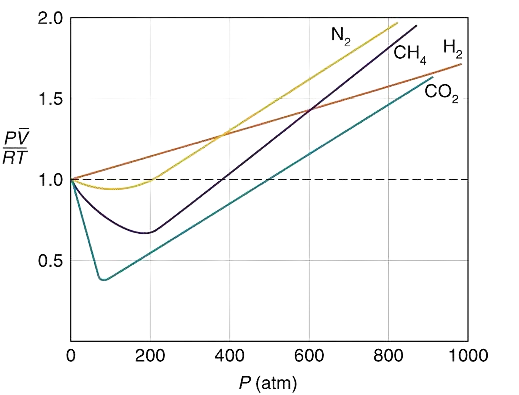
\includegraphics[scale=.5]{nitro.png}
	\end{minipage}		
	
	\begin{mdframed}[backgroundcolor=brown!10]  
	Como el factor de compresibilidad de un gas ideal vale $Z=1$, el gas que más se acerque a la línea horizontal punteada será el que tenga el comportamiento más ideal. A $400\;K$ el metano es el gas que mejor se describe con esta modelización.
\end{mdframed}		
    	\end{itemize}
    \qed 
\end{enumerate}

\end{document}

